%%%%%%%%%%%%%%%%%%%%%%%%%%%%%%%%%%%%%%%%%%%%%%%%%%%%%%%%%%%%%%%%%%%%%%%%%%%%%%%%
% Template for USENIX papers.
%
% History:
%
% - TEMPLATE for Usenix papers, specifically to meet requirements of
%   USENIX '05. originally a template for producing IEEE-format
%   articles using LaTeX. written by Matthew Ward, CS Department,
%   Worcester Polytechnic Institute. adapted by David Beazley for his
%   excellent SWIG paper in Proceedings, Tcl 96. turned into a
%   smartass generic template by De Clarke, with thanks to both the
%   above pioneers. Use at your own risk. Complaints to /dev/null.
%   Make it two column with no page numbering, default is 10 point.
%
% - Munged by Fred Douglis <douglis@research.att.com> 10/97 to
%   separate the .sty file from the LaTeX source template, so that
%   people can more easily include the .sty file into an existing
%   document. Also changed to more closely follow the style guidelines
%   as represented by the Word sample file.
%
% - Note that since 2010, USENIX does not require endnotes. If you
%   want foot of page notes, don't include the endnotes package in the
%   usepackage command, below.
% - This version uses the latex2e styles, not the very ancient 2.09
%   stuff.
%
% - Updated July 2018: Text block size changed from 6.5" to 7"
%
% - Updated Dec 2018 for ATC'19:
%
%   * Revised text to pass HotCRP's auto-formatting check, with
%     hotcrp.settings.submission_form.body_font_size=10pt, and
%     hotcrp.settings.submission_form.line_height=12.5pt
%
%   * Switched from \endnote-s to \footnote-s to match Usenix's policy.
%
%   * \section* => \begin{abstract} ... \end{abstract}
%
%   * Make template self-contained in terms of bibtex entires, to allow
%     this file to be compiled. (And changing refs style to 'plain'.)
%
%   * Make template self-contained in terms of figures, to
%     allow this file to be compiled. 
%
%   * Added packages for hyperref, embedding fonts, and improving
%     appearance.
%   
%   * Removed outdated text.
%
%%%%%%%%%%%%%%%%%%%%%%%%%%%%%%%%%%%%%%%%%%%%%%%%%%%%%%%%%%%%%%%%%%%%%%%%%%%%%%%%

\documentclass[letterpaper,twocolumn]{article}

\usepackage{style}

% to be able to draw some self-contained figs
\usepackage{tikz}
\usepackage{amsmath}

% inlined bib file
\usepackage{filecontents}

\usepackage{setspace}
\linespread{1.25}

%-------------------------------------------------------------------------------
\begin{filecontents}{\jobname.bib}
%-------------------------------------------------------------------------------
@Book{arpachiDusseau18:osbook,
author =       {Arpaci-Dusseau, Remzi H. and Arpaci-Dusseau Andrea C.},
title =        {Operating Systems: Three Easy Pieces},
publisher =    {Arpaci-Dusseau Books, LLC},
year =         2015,
edition =      {1.00},
note =         {\url{http://pages.cs.wisc.edu/~remzi/OSTEP/}}
}
@InProceedings{waldspurger02,
author =       {Waldspurger, Carl A.},
title =        {Memory resource management in {VMware ESX} server},
booktitle =    {USENIX Symposium on Operating System Design and
Implementation (OSDI)},
year =         2002,
pages =        {181--194},
note =         {\url{https://www.usenix.org/legacy/event/osdi02/tech/waldspurger/waldspurger.pdf}}}
\end{filecontents}

\newcommand{\vrsdust}[1]{
\includegraphics[height=#1]{redstone_dust.png}}
% \newcommand{\vrswire}[1]{\includegraphics[height=#1]{redstone_wire.png}}

\newcommand{\txtrsdust}{\vrsdust{0.55cm} \hspace{0.1in}}
% \newcommand{\txtrswire}{\vrswire{0.6cm}


%-------------------------------------------------------------------------------
\begin{document}
%-------------------------------------------------------------------------------

%don't want date printed
\date{}

% make title bold and 14 pt font (Latex default is non-bold, 16 pt)
\title{\Large \bf \vrsdust{0.7cm} \hspace{0.1in} Redstone: a Deterministic Simulation Testing Framework for Distributed Systems}

%for single author (just remove % characters)
\author{
{\rm Benjamin Friedman}\\
% Your Institution
\and
{\rm Katherine Li}\\
% Second Institution
\and
{\rm Matthew Mattei}\\
\and
{\rm Ron Dubinsky}\\
% copy the following lines to add more authors
% \and
% {\rm Name}\\
%Name Institution
} % end author

\maketitle

%-------------------------------------------------------------------------------
\begin{abstract}
%-------------------------------------------------------------------------------
{\fontsize{12}{15}\selectfont 
In testing distributed systems,
confirming a system's tolerance of faults in disks and networks is not only useful but necessary.
Redstone, a deterministic simulation testing framework,
amplifies failures in various substrates underlying a distributed system
in order to confirm the system's ability to withstand these failures.
We intercept calls to the kernel for the disk and the network, as well as to clock functions,
introducing our own code. Our control over clock functions further allows us to
``accelerate'' time, %NOTE: what the fuck
increasing ability to test faster, and to emulate the effects of clock jitter. Additionally, our framework has been made modular to be easily implemented alongside nearly any distributed system for the sake of enabling testing a breadth of distributed systems. Most importantly, though, Redstone's
determinism allows reproduction of failure conditions,
allowing developers to confirm, having encountered and debugged a failure,
that their system will not fail again when confronted by identical conditions. By basing program flow on a pre-chosen seed, any found faults, no matter how improbable, can be reliably replicated. We implement and evaluate our framework on a simple system in Linux to demonstrate this determinism in practice.

}
\end{abstract}


%-------------------------------------------------------------------------------
\section{\txtrsdust Introduction}
%-------------------------------------------------------------------------------

{\fontsize{12}{15}\selectfont 
Distributed systems are complicated ones,
because they rely not only on the particular machines
on which the systems run but also on the network connecting these machines.
As such, distributed systems must contain many
(often complicated and difficult-to-reason-about)
mechanisms by which to recover from both network and machine failures
(more specifically, network latency, disk I/O failure, bugs in the kernel,
and all manners of timing-based bugs).

Distributed systems often run on comparatively long time-scales:
a system may be running for months or years,
hopefully without failure.
However,
it is unrealistic to spend months testing a system to confirm that such durations will not lead to failure.
But, with control of the machine's time system calls,
we can effectively "accelerate" time in the test,
meaning the distributed system to be tested will act as though it has been running for such a duration,
without interrupting development for such an extended period of time. 

Additionally, distributed systems are highly varied,
and as a result may require features or platform support not foreseen by our implementation.
Modularity in our design allows our framework to be easily extended,
not future-proofing it but allowing it to be future-proofed.

Testing offers the ability to confirm that a system can withstand failures.
Specifically, if one can introduce a failure and check that the system withstands it,
it certainly increases the degree of trust in the system.
However, in order to be effective,
such testing must be able to consistently introduce failures.
Just hoping that failures naturally occur in the process of testing is a non-starter;
they must be introduced.
In order to introduce failures, the system must have control of the network, disk,
and time systems on which a distributed system relies.
Therefore, the system must simulate this functionality whilst also injecting failure where possible.

``Consistently" is the key phrase here,
as a test must be replicable.
A good testing system must not only introduce failures,
but be able to repeatedly introduce exactly the same failures in exactly the same way.
In the words of John Ousterhout,
``the only thing worse than a problem that happens all the time is a problem that doesn't happen all the time."
Therefore, our system must be \textit{deterministic}. To that end, our system has been designed around deterministic replication of program flow and results.

}

\section{\txtrsdust Related Work}
% Redstone was inspired by work done by the TigerBeetle team,
% and their work in testing the TigerBeetle database.
% However, the limitation of their work is that their simulator is compiled specifically for their software.

{\fontsize{12}{15}\selectfont 
Although their work is not a research paper,
the TigerBeetle team has provided inspiration to Redstone in their work developing a testing system for their database.
This work heavily involved hastened testing of simulated distributed system faults.
However, a significant limiting factor in their work as compared to ours is that the simulator is compiled specifically for the software being tested.
While this setup works for their well-abstracted code that they can freely recompile to embed the simulation,
there are many, many more distributed systems in the real world that this form of simulation suits poorly at best.

As such, we wanted to try to emulate the idea on which they built their replicator.
The basis of their simulator involves mocking all input and output:
their work includes a network simulator to force network faults and latencies,
and an in-memory storage simulator to force storage faults and latencies.
The simulator then speeds up the clock to make I/O operations occur far more frequently than in production,
causing faults that may only occur once a year, or even more infrequently, to occur in a matter of days.
Such functionality would be highly valuable in testing nearly any production distributed system.

Therefore,
we wanted to develop a framework that incorporates a number of features from the basic simulation methodologies
TigerBeetle’s simulator includes (namely, hastened I/O faults for network and in-memory storage),
but one that can be generally implemented on normal systems and run a much broader range of applications.

}

\section{\txtrsdust Architecture}

\begin{figure}
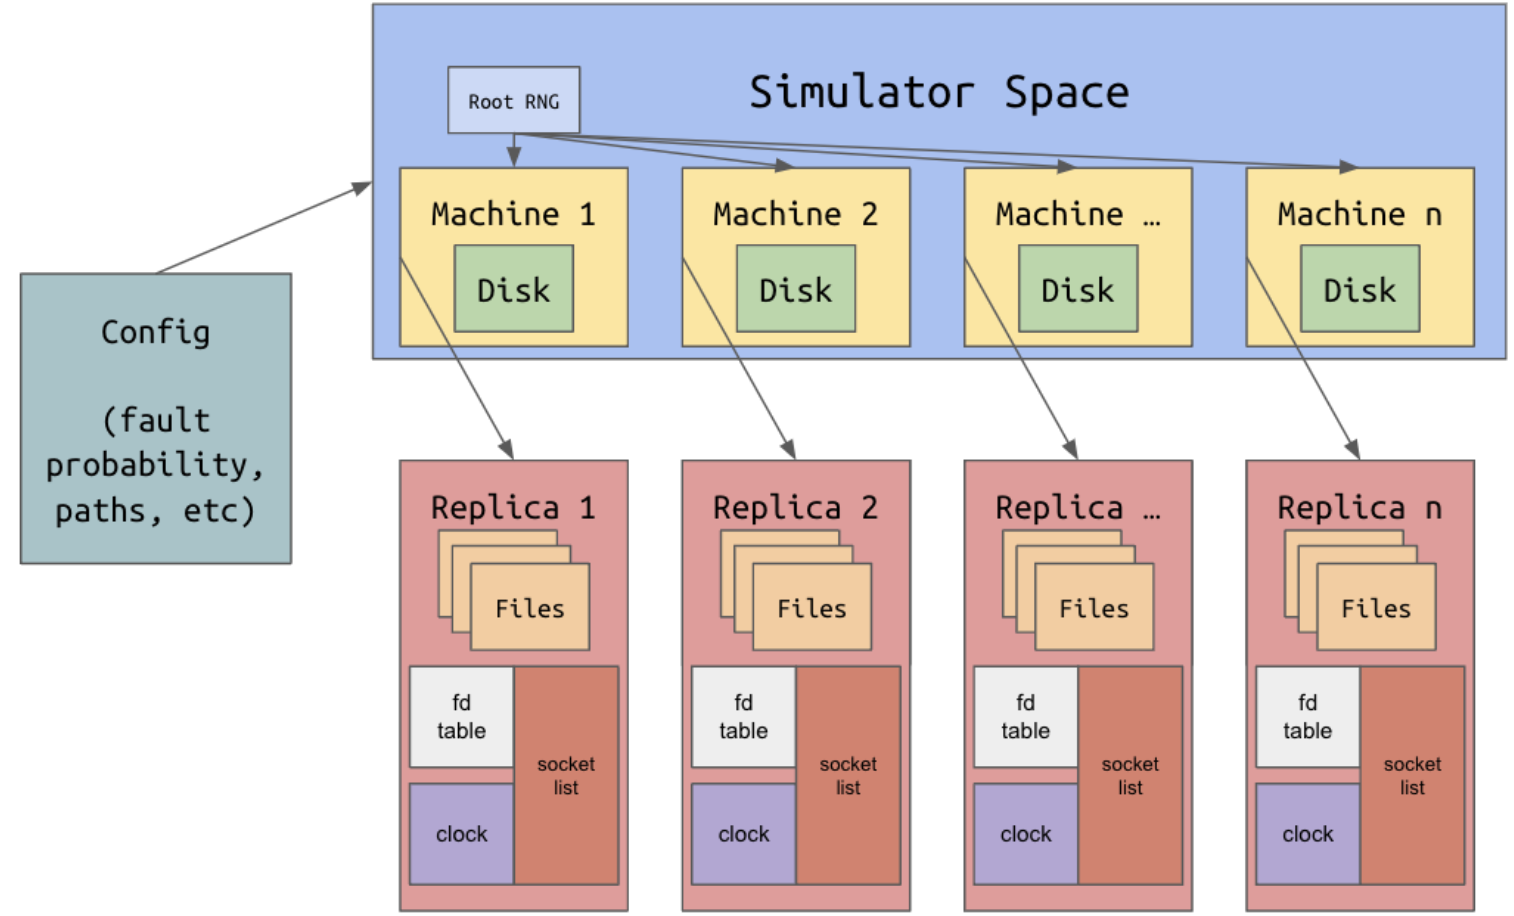
\includegraphics[width=0.45\textwidth]{redstone_architecture.jpeg}
\caption{General architecture of the Redstone framework}
\end{figure}

{\fontsize{12}{15}\selectfont 
Figure 1 provides a visual representation of the architecture powering Redstone.
The region marked "simulator space" represents the simulator process,
for which system calls are re-routed to the syscall implementations specified for the simulator run.
Within the simulator process there are multiple “machines”,
representations of physical machines that, in production, would actually be different machines.
Each of these machine abstractions have their own simulated disk space.
Each machine abstraction is associated with a child process,
called a “replica”,
of the simulator process that runs the actual functionality expected of the individual machine,
working with the machine’s “files” (the in-memory storage mocked up by the simulator).

}

\section{\txtrsdust System Call Interception}

{\fontsize{12}{15}\selectfont 
In order for Redstone to perform its role of replacing the implementation of system calls,
we need some method of intercepting calls made to the system library and,
conditional on whether we seek to alter their behavior,
replacing them.

Initially, we planned to use \texttt{LD\_PRELOAD},
a feature of the dynamic linker,
which allows a user-created shared library to override weakly linked \texttt{libc} symbols on process start.
Unfortunately,
\texttt{LD\_PRELOAD} is often finicky and can be unreliable,
as we saw in our own attempts to use it,
causing us to opt not to employ it and to instead seek alternatives.
One option was to simply link in a static library containing all the overridden functions.
This would have meant that the targeted program would need to be compilable specifically for use with Redstone.
This was decided to be a barrier to the goal of easy simulation without code changes to the program to be tested,
so we opted for the second fallback: the \texttt{ptrace(2)} system call.

\texttt{ptrace(2)} is used by debuggers to fully control a child process,
which gives the user a lot of power over the simulated processes.
Unfortunately,
with great power came a significant amount of overhead.
Using the \texttt{PTRACE\_SYSCALL} request,
Redstone runs the program until a syscall instruction is issued,
at which point it accepts the arguments,
the syscall number, and some other state.
We pass this information, as well as the syscall identifier,
to a platform-agnostic hooks table that, if possible,  calls the relevant hook.
If no hook is present for the given syscall,
Redstone passes the syscall through to the kernel and continue the program's execution.
If a hook is present for the given syscall,
and returns that it has successfully handled the given request,
Redstone first replaces the syscall number with that of \texttt{getpid}
(a cheap syscall that doesn’t take any arguments and has no side effects),
then changes the program registers to replace the syscall return value with our result.
For obvious reasons, this is quite slow.
The \texttt{PTRACE\_SYSEMU} command
(which just doesn’t execute the system call, allowing us to set the return value instead)
can reduce this overhead,
but not by any meaningful amount.
We have more data on the specific overheads imposed by the \texttt{ptrace} runner in the evaluation section.

Aside from the overheads imposed by \texttt{ptrace},
there is an additional limitation:
Linux implements some system calls in userspace dynamic libraries for improved performance.
The modern version of this is known as \texttt{vDSO},
and unfortunately is not caught by \texttt{PTRACE\_SYSCALL}.
To counter this, we forcefully disable the use of \texttt{vDSO} on simulated programs upon start,
falling back to traditional system calls.
This further worsens the overheads of \texttt{ptrace}.

Owing to the platform-specific nature of interception,
this part of Redstone is confined to black magic jail,
and can be easily overridden to boost platform support or improve performance.
For example,
if ever \texttt{LD\_PRELOAD} decided to stop being so temperamental,
effectively only one line of code would need to be changed in order to replace the simulator’s runner with a different implementation.

}

\section{\txtrsdust System Call Interception Coverage}

{\fontsize{12}{15}\selectfont 
In the process of implementing Redstone,
we have encountered limitations to the extent and nature of what we can properly intercept and handle.
These fall into three categories:
that coverage which may be attained with sufficient work,
that coverage which is conditionally possible depending on the workload,
and that which is impossible.

The first category,
that coverage which may be attained with sufficient work
contains features like \texttt{epoll}, \texttt{select}, \texttt{poll}, \texttt{io\_uring},
more exotic network protocols,
and additional fault classes and more sophisticated fault injection algorithms.
These can be implemented given sufficient additional time investment.

The second category,
that coverage which is conditionally possible depending on the workload,
is more interesting, and perhaps the most common example is that of \texttt{getrandom}.
Given that Redstone's entire reason for existence is to be as deterministic as possible,
the naive approach would be to forward to a simulated CPRNG, such as ChaCha20,
that is seeded by some derivation of the simulation seed.
Unfortunately, if a program uses randomness for cases like cryptographic key generation,
and any kind of external accesses occur,
this indicates the presence of a significant security vulnerability due to reused keys.
As such,
randomness remains unimplemented,
and should only really be implemented assuming we can guarantee that a vulnerability will not occur on a given program.

The third category,
that which is impossible,
is introduced by restrictions on userspace.
\texttt{mmap} is the prime example of this category.
We have no way of replacing the page-in/page-out handling so this is also left as a passthrough. 

}

\section{\txtrsdust Randomness and Determinism}

{\fontsize{12}{15}\selectfont 
The core of the simulated testing framework is its test injection.
By introducing randomness into whether or not a network packet is dropped or replayed,
for example, the system is able to cover a breadth of ``environmental conditions",
so to speak,
that are harder to anticipate when designing the distributed system.

Many of these ``environmental conditions"
will inevitably cause failures in the distributed system due to insufficient edge case handling by the implementers of the system.
This is a feature, not a bug.
The whole purpose of distributed systems testing frameworks is to find these cases.

The primary goal of Redstone, however,
in addition to revealing these cases,
is to make it simple to be able to deterministically find these “random” cases.
The method by which Redstone seeks to do so is by introducing a seed.

The seed is chosen by the user before the simulator runs.
Wherever randomness is necessary
% Then, rather whenever a random number is called in the simulation
(say, to determine whether a packet should be dropped),
the value can be pseudo-randomly generated based on the seed.

Thus, the system performs a ``random" and yet totally deterministic program flow,
which can be used in development for iteration on the tested system.
When an interesting program flow is discovered by the user,
instead of just relying on logs after the fact,
the user can take note of the seed with which the simulation was run and simply run it again.

Due to the guarantees provided by the seed, the execution of the program flow, and the interactions between the two,
the user can expect the exact same program flow to execute and to reproduce the same sequence of events as the one they see in their logs.
Between these logs and the replicability of the program flow results,
the user is able to get the randomness desired of a distributed system testing framework as well as the determinism required to understand and replay the results.

}

\section{\txtrsdust Evaluation}

{\fontsize{12}{15}\selectfont 
\texttt{NOTE: we are in the process of writing up this section, and will submit this in an amended version of the writeup tomorrow morning.}
% This section needs: at least 1 graph/table, explanations of what we evaluated and how, what the evaluation tells us.

}

\section{\txtrsdust Conclusion}

{\fontsize{12}{15}\selectfont 
\texttt{NOTE: we are in the process of writing up this section, and will submit this in an amended version of the writeup tomorrow morning.}
% Based on our results, we find the Redstone framework promising in its ability to deterministically replay results. 

% // Talk about limitations, otherwise desired future plans/potential future work

}

% Distributed systems are fucking stupid.
% 
% Therefore, in order to combat this stupidity, there was the advent of a concept of "testing".
% This dark and arcane art is wonderfully usable but falls flat when tested conditions occur only
% rarely. The best example of such wild conditions are things like network latencies, disk
% io errors, kernel bugs, time, and more. Everything has some level of doing a fucky wucky,
% so our job is to make these fucky wuckies happen more often so that programmers are better able to
% understand how their system handles such fucky wuckies

% %-------------------------------------------------------------------------------
% \section*{Acknowledgments}
% %-------------------------------------------------------------------------------
% 
% The USENIX latex style is old and very tired, which is why
% there's no \textbackslash{}acks command for you to use when
% acknowledging. Sorry.
% 
% %-------------------------------------------------------------------------------
% \section*{Availability}
% %-------------------------------------------------------------------------------
% 
% USENIX program committees give extra points to submissions that are
% backed by artifacts that are publicly available. If you made your code
% or data available, it's worth mentioning this fact in a dedicated
% section.

%-------------------------------------------------------------------------------
\bibliographystyle{plain}
\bibliography{\jobname}

%%%%%%%%%%%%%%%%%%%%%%%%%%%%%%%%%%%%%%%%%%%%%%%%%%%%%%%%%%%%%%%%%%%%%%%%%%%%%%%%
\end{document}
%%%%%%%%%%%%%%%%%%%%%%%%%%%%%%%%%%%%%%%%%%%%%%%%%%%%%%%%%%%%%%%%%%%%%%%%%%%%%%%%

%%  LocalWords:  endnotes includegraphics fread ptr nobj noindent
%%  LocalWords:  pdflatex acks
